
\documentclass{acm_proc_article-sp}

\usepackage{amsmath}
\usepackage{verbatim}
\usepackage{textcomp}
\usepackage{graphicx}
\usepackage{subcaption}
\usepackage{url}
\usepackage{multicol}
\usepackage{tikz}
\usetikzlibrary{positioning}
\usepackage{wasysym}


\begin{document}

\title{Difficult Handwritten Digit Classification \\
{\normalsize Code available at: \url{https://github.com/slflmm/Miniproject-3}}} 
\subtitle{COMP 598 -- Miniproject 3 -- Team X}

\numberofauthors{3} 
\author{
% 1st. author
\alignauthor 
Narges Aghakazemjourabbaf\\
	\affaddr{260460855}
\alignauthor
Stephanie Laflamme\\
	\affaddr{260376691}
% 2nd. author
\alignauthor Benjamin La Schiazza\\
	\affaddr{260531181}
% 3rd. author
}

\date{Oct15}



\maketitle
\begin{abstract}

\end{abstract}

\section{Introduction}% overview of approach
The MNIST dataset--a collection of labelled handwritten digits, obtained from American Census Bureau employees and high school students\cite{LeCun2}--has been widely used as a benchmark in machine learning. However, handwritten digit recognition in the style of the MNIST dataset can very well be considered a solved problem; indeed, the best learners achieve near-human performance at correctly labelling new digits\cite{Ciresan}, obtaining a peak accuracy of $99.79\%$\cite{Wan}.

Bringing back the challenge of handwritten digit recognition, researchers at Universit\'{e} de Montr\'{e}al introduce noise to MNIST images to form a new dataset for difficult handwritten digit classification. Images are enlarged from $28\times28$ to $48\times48$ pixels, digits are embossed, textures from a large variety are added to the images' backgrounds, and digits are rotated by random amounts.

In the context of an in-class competition, we tackle this dataset. In this paper, we report results with four classifiers; a perceptron, a fully-connected neural network, a linear SVM model, and a convolutional neural network. Moreover, when appropriate, we consider three feature sets; raw pixels, PCA features, and features derived from Gabor filters. We describe our learners and features in depth in the early sections of this report, and follow-up with a description of our methodology and results. We end with a discussion of the implications of our findings.


\section{Algorithm Selection}% for each category
As our preprocessing treatment and feature sets vary between our choices of learning algorithms, we introduce the four here; we use a perceptron, a fully-connected neural network, a linear SVM, and a convolutional neural network.

\subsection{Perceptron}
We implement a multiclass perceptron as a baseline classifier. Given $n$ examples with $m$ features each, and given $k$ classes, the perceptron learns a matrix $W$ of $(m+1) \times k$ weights (one weight for each feature-class combination, and a bias vector) by gradient descent on the error $$Err(x) = (y - f(W^Tx)),$$
where $f$ is the Heaviside step function, $x$ is an example, and $y$ is its class.

\subsection{Fully-Connected Neural Network}
The fully-connected neural network, also known as a multilayer perceptron, concatenates layers of perceptrons, but uses a softer activation function than the step function. The advantage of this arrangement over a single layer is that complex, non-linear functions can be learned; for instance, a linear learner cannot encode the XOR function, but a neural network can do it with only two layers. Our implementation uses the easily differentiable sigmoid, written $$\sigma(z) = \cfrac{1}{1 + e^{-z}}.$$ The weights of each layer are learned by gradient descent on the error, $$Err(x) = y - h_w(x),$$ where $h_w(x)$ is the network's current guess for the label of example $x$ and $y$ is its true label.

\subsection{Linear SVM}
We use the scikit-learn \cite{scikit-learn} library's `SVC' implementation of a linear SVM (support vector machine). This learning algorithm solves the quadratic optimization problem written as
\begin{align*} 
\hbox{arg} \min_{w,b} \|w\|^2 \\
\hbox{subject to } y_i(w \cdot x_i - b) \geq 1,
\end{align*}
where $w$ is the normal vector to the hyperplane separating two classes. It handles the dataset's multiple classes using a `one-vs-the-rest' approach.

\subsection{Convolutional Neural Network}
Although fully-connected neural networks tend to perform very well at machine learning tasks, their ability to classify images is sensitive to shifts in position or shape distortions--they can be bad at identifying invariant patterns. In the early '80s, Fukushima introduced convolution layers to remedy that problem by handling geometrical similarities regardless of position.\cite{Fukushima} A convolution applies a filter to an image; a convolution layer contains many such filters, whose values are learned as the neural network is trained. This serves as an implicit, learned feature extraction at the start of the neural network, typically followed by hidden layers.

The use of convolution layers seem particularly appropriate given the difficulty of our dataset, which adds noise-inducing modifications to the MNIST dataset. Indeed, LeCun has shown that a convolutional neural network trained with MNIST images continues to predict digits correctly regardless of rotations and noise.\cite{LeCun}

We note that neural networks with many layers tend to overfit; there may be many complicated relationships between examples and their labels, and enough hidden units to model these relationships in multiple ways. Hinton et al.\cite{Hinton} introduced the concept of dropout to alleviate this issue. During training, hidden units are randomly omitted with probability $p$, which helps prevent complex co-adaptations on training data. 

The application of dropout to convolutional neural network has been successfully applied; Krizhevsky et al. applied dropout to the hidden layer weights of their convolutional neural network, and vastly outperformed other methods on an ImageNet classification competition.\cite{Krizhevsky} 

In light of these findings, we implement our own convolutional neural network. Its architecture consists of a variable number of convolution layers, followed by a variable number of hidden layers and the output layer. We apply dropout to the hidden layers, and train our network using minibatch SGD. We also experiment with the use of learning rate decay and momentum.

\section{Preprocessing}
The raw pixels are normalized. In the case of the perceptron, fully-connected neural network, and linear SVM learners, they are standardized. For each example $i$ in the training set, and each feature $j$, we replace features with their standardized value $$x'_{ij} = \cfrac{x_{ij} - \mu_{j}}{\sigma_{j}},$$ where $\mu_j$ is the average value for feature $j$ and $\sigma_j$ is its standard deviation. These values for $\mu_j$ and $\sigma_j$ are subsequently used to apply the same transformation to the test set examples.

For the convolutional neural network, we apply local contrast normalization; given a $48\times48$ image $X$ from the dataset, we let $$X = \cfrac{256\times (X - X_{min})}{X_{max} - X_{min}},$$ where $X_{max}$ and $X_{min}$ are the maximum and minimum values in $X$'s pixels, respectively. 

\section{Feature Design and Selection}
When appropriate for the learner, we consider three feature sets; standardized raw pixels, PCA, and Gabor filter-based features. For the open method, we consider contrast-normalized raw pixels and the addition of rotation-perturbed examples.

\subsection{Pixels}
We use the post-preprocessing pixel information as a baseline feature set.This produces feature vectors of length 2304. 

\subsection{PCA}
Principal component analysis (PCA), developed by Pearson in the early 1900s\cite{Pearson}, converts a set of possibly correlated features into a linearly uncorrelated representation, with the resulting features ordered by variance. 

We use the implementation of PCA provided by the Scikit-learn library\cite{scikit-learn}, which uses singular value decomposition of the input data matrix.

As removing the least useful features made the results of our baseline classifier worse, we keep full dimensionality. However, we expect PCA features to produce better results given that they are linearly uncorrelated.

\subsection{Gabor}
Gabor filters are linear filters used for edge detection and are thought to be similar to the early stages of visual processing in humans. Their frequency and orientations correspond roughly to simple cells in the visual cortex of humans and other mammals; these cells can be modelled with Gabor functions.\cite{Jones}\cite{Marvcelja} As these filters are well-suited to image processing, we attempt to translate them into features.

We use two kinds of Gabor filters: for the perceptron and fully-connected neural network, we use a simplified expression due to lack of time and memory; we describe these features in more detail below. For the linear SVM model, we take advantage of scikit-learn's online learning capacity and use as features the pixels of the results of convolving each filter with an image.

Previous research has used the energy of the convolution between a Gabor filters and image (a measure of how strongly the filter responds to that image\cite{Grigorescu}) as a feature by summing its magnitudes in the image.\cite{Bau} This is equivalent to using the Frobenius norm of the convolved image as a feature. 

Using the Scikit-learn library\cite{scikit-learn}, we generate 16 Gabor filters with 8 equidistant $\theta$ values, $\sigma = \{1, 3\}$, and frequencies $= \{0.05, 0.25\}$. Figure \ref{fig:gabor} illustrates the effects of $\theta$, $\sigma$, and frequency with a sample of our filters. We form the feature vector of an image in the dataset by collecting the Frobenius norms of the image convolved with each filter. 

\begin{figure}[h]
	\centering
	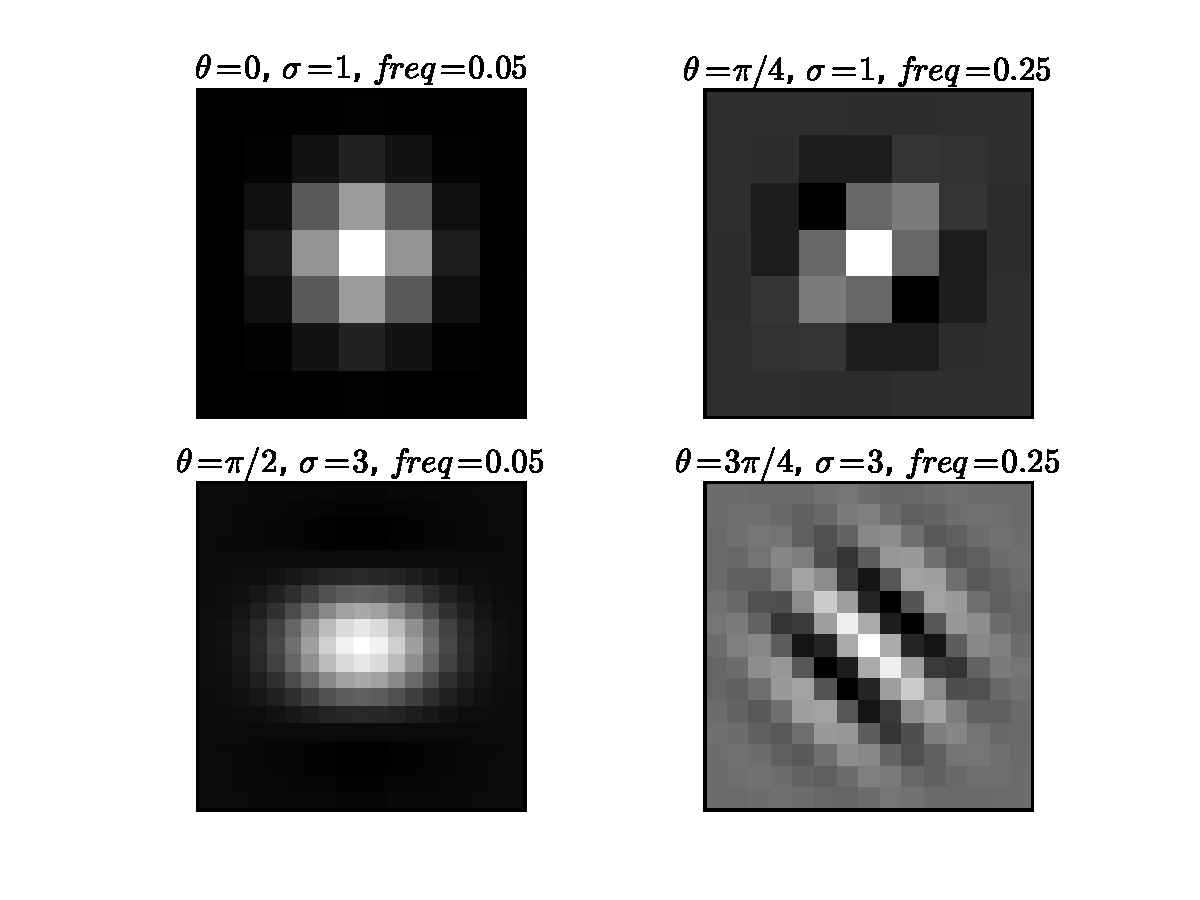
\includegraphics[width=\linewidth]{gabors}
  	\caption{Some Gabor filters}
  	\label{fig:gabor}
\end{figure}



\section{Optimization} 
Given the vast amount of time required to train a convolutional neural network, we implement ours to run on a GPU. This reduces the training time by approximately a factor of 10. We use Theano\cite{Theano}, a symbolic Python library that compiles computation-heavy functions in C and can execute them on a GPU. We use the cuda-convnet implementation of convolutions\cite{Krizhevsky}, which offers a 3-fold speed improvement relative to Theano's convolution function.

\section{Parameter Selection Method}% model order, learning rate, etc
For each learner, we fix the hyperparameters to compare the performance of appropriate feature sets, and perform a preliminary manual inspection to identify viable hyperparameters, followed up by either the traditional gridsearch, or a random search. In cases where there are many hyperparameters and training is long, random search offers a faster alternative to gridsearch for finding good hyperparameters. It has been shown to obtain results as good as or better than gridsearch\cite{Bergstra}. The details of parameter selection are discussed in this section.

\subsection{Perceptron}
The perceptron can use pixel, PCA, or Gabor features. We initially fix the hyperparameters to identify the most promising feature set using 5-fold cross-validation. We then consider its two hyperparameters--learning rate and number of learning iterations--and perform gridsearch for $\alpha \in [10^{-4},10^{-1}]$ and the number of iterations ranging form 10 to 35; the averaged validation accuracy from 5-fold cross-validation is used as a measure of success for the hyperparameter setting. 

\subsection{Fully-Connected Neural Network}
The neural network can also use pixel, PCA, or Gabor features. As we did for the perceptron, we fix what appear to be reasonable hyperparameters and identify the best feature set for this classifier; we use results from 2-fold cross-validation, as neural networks take a long time to train. Then, we perform random search over 15 hyperparameter settings; we use mean accuracy from 2-fold cross-validation to determine the most promising parameter setting. Table \ref{tab:nn-hyp} lists the hyperparameters and the range of values we consider.
\begin{table}[h!]
  \centering
  \begin{tabular}{|l|l|}
    \hline 
    {\bfseries Hyperparameter} & {\bfseries Values}\\
    \hline \hline
    Number of layers & \{1, 2\} \\
    Hidden units per layer & \{10, 15, ..., 30\} \\
    Learning rate & $[0.0001, 0.1]$ \\
    \hline
  \end{tabular}
  \caption{Neural network hyperparameters and their considered values}
  \label{tab:nn-hyp}
\end{table}


\subsection{Linear SVM}
As we do for the perceptron and fully-connected neural network, 


\subsection{Convolutional Neural Network}
The only appropriate features for a convolutional neural network are pixel features. We must optimize many hyperparameters; in addition to those for the fully-connected neural network, we must also consider the dropout rate, as well as the number of convolution layers, the number of filters per layer, and the filter sizes. We must also consider activation functions, learning rate decay, and momentum rate. 

Due to time constraints, we can only sample a small portion of this very large parameter space. Hence, we select hyperparameters with manual search and train models until they reach a validation accuracy plateau to compare their performance. It should be noted that, due to time concerns, we simply use 10\% of the training data as a validation set rather than our usual cross-validation method.

We start from the parameters used in Theano's convolutional network tutorial, where they train a network on the MNIST dataset. That is, we start with two convolutional layers with 20 and 50 filters respectively, each with filter sizes $5\times 5$. We use a learning rate $\alpha = 0.1$, without momentum, learning rate decay, or the extended dataset. From there, we apply modifications to each parameter and attempt to find a good model.

Luckily, we can use heuristics to reduce search when it comes to the size of hidden layers and the size and number of filters per convolution layer. We keep in mind tips and tricks offered by Theano's deep learning tutorials\cite{Theano-tut}:
\begin{itemize}
\item When filter size increases, number of filters decrease; this is to preserve information across convolution layers. 
\item $5 \times 5$ filters in the first convolution layer work well with the MNIST dataset of size $28 \times 28$ pixels, while filter sizes of $12\times12$ or $15\times15$ work well with images with hundreds of pixels in each dimension.
\end{itemize}

\section{Testing and Validation}%detailed analysis of results

\subsection{Perceptron}
In a primary step, we performed 5-fold cross-validation to compare raw pixels, PCA, and Gabor features using a fixed learning rate ($\alpha = 0.01$) and number of iterations (15). As shown in Table \ref{tab:perc-features}, PCA features were the most performant, with a validation accuracy of 26.282\%.
\begin{table}[h!]
  \centering
  \begin{tabular}{|c||c|c|c| }
    \hline
    {\bfseries Features} & Pixels & PCA & Gabor \\
    \hline
    {\bfseries Accuracy} & 25.794 & 26.282 & 10.398 \\
    \hline
  \end{tabular}
  \caption{Mean validation accuracy of perceptron using different features}
  \label{tab:perc-features}
\end{table}

Using PCA features, we performed 5-fold cross-validation over the learning rate $\alpha$ and the number of training iterations of the perceptron model. Figure \ref{fig:perc-gridsearch} shows the results of gridsearch with both parameters. The precise values of the best parameters found by the gridsearch cross-validation procedure were $\alpha = 0.0005$ with 25 training iterations, yielding a mean validation accuracy of 26.598\%.\footnote{Additional results showing training error vs validation error are shown in Appendix \ref{sec:additional-results}}
\begin{figure}[h!]
	\centering
	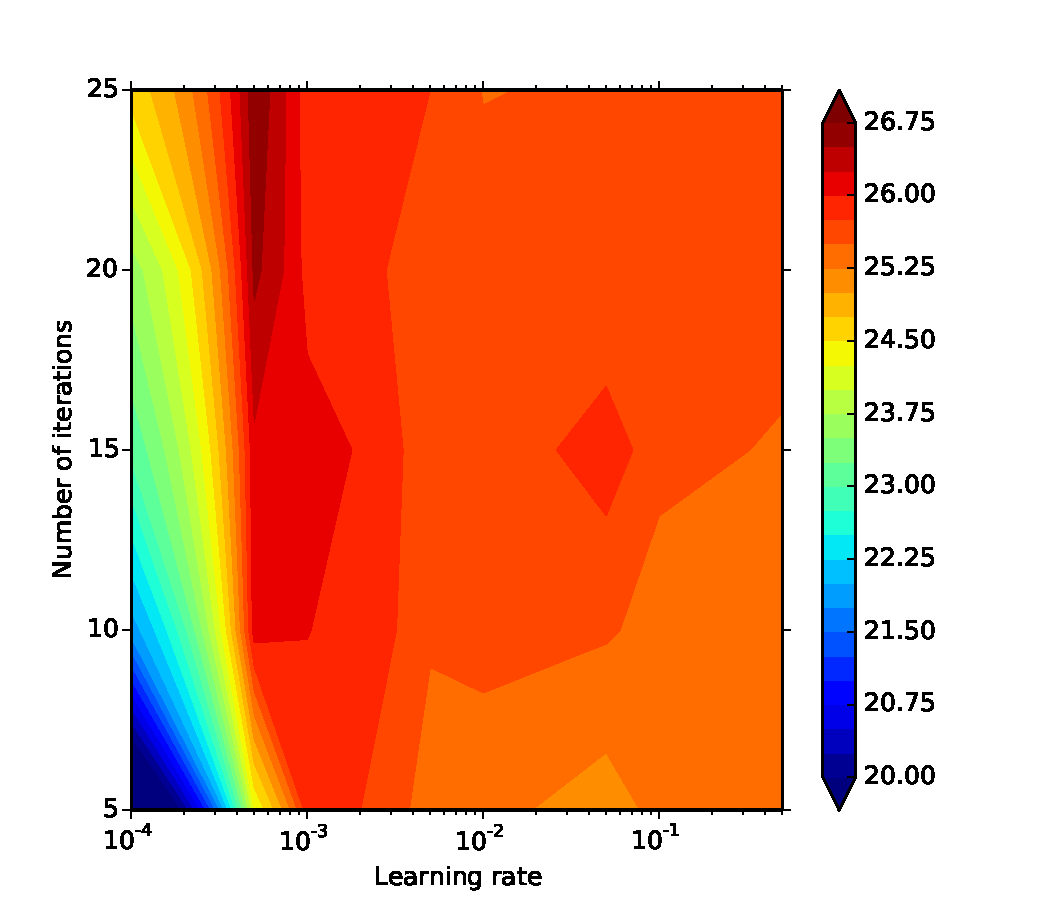
\includegraphics[width=\linewidth]{perceptron_gridsearch}
  	\caption{Mean cross-validation accuracy as a function of parameters $\alpha$ and number of iterations}
  	\label{fig:perc-gridsearch}
\end{figure}

After training our perceptron on the complete training set using these parameters, we submitted our results to Kaggle and obtained a test accuracy of 27.420\%. As an approximation of the test confusion matrix, we provide the confusion matrix for the combined validation sets in Figure \ref{fig:perc-confusion}. Note the perceptron's greater ability to identify 0s and 1s compared to other digits.
\begin{figure}[h!]
	\centering
	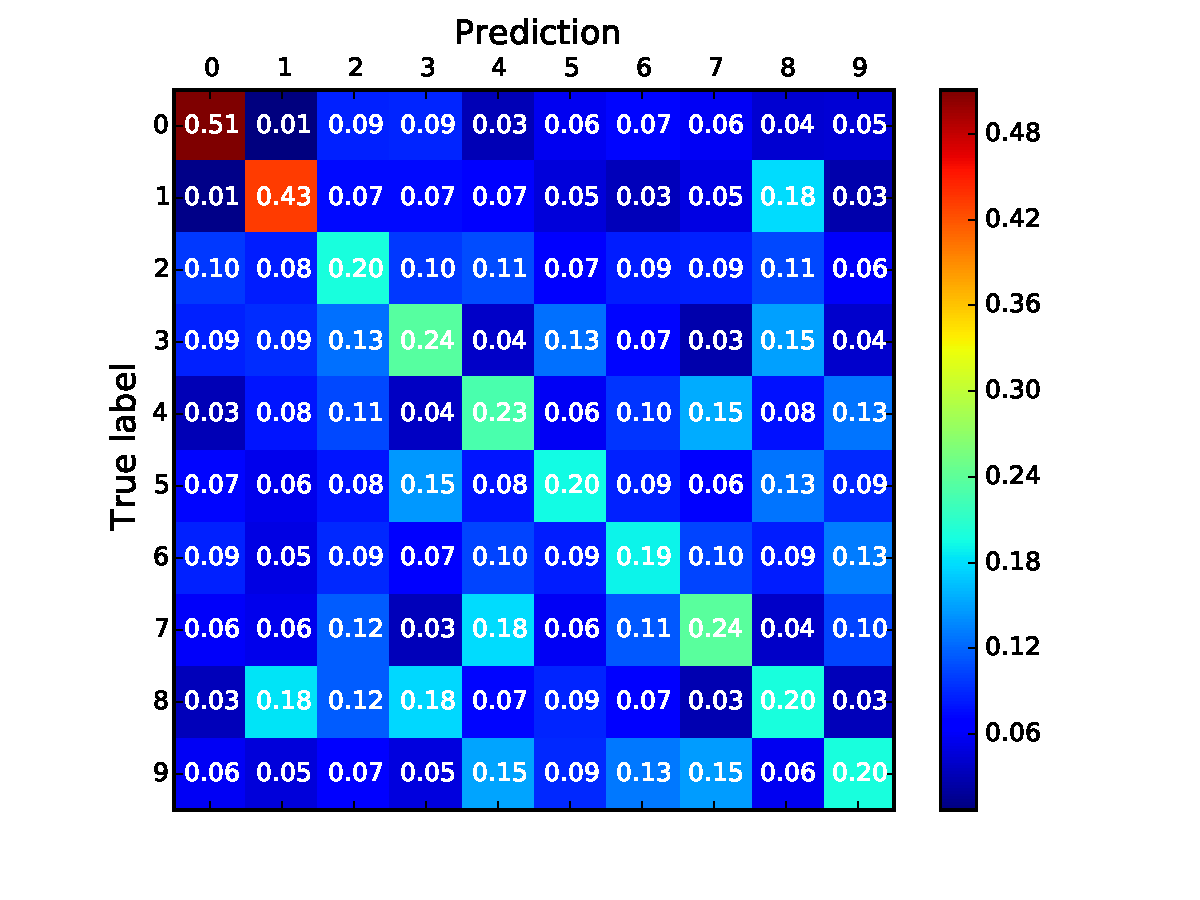
\includegraphics[width=\linewidth]{perceptron_confusion}
  	\caption{Validation confusion matrix for perceptron}
  	\label{fig:perc-confusion}
\end{figure}

\subsection{Fully-Connected Neural Network}
To select the best feature set for this classifier, we performed a quick 2-fold cross-validation with each feature set, setting $\alpha = 0.01$, with one layer of 15 hidden units, and training for 10 epochs. Table \ref{tab:nn-features} shows the mean validation accuracies of each feature set; standardized pixel features performed best with 32.570\% accuracy.

\begin{table}[h!]
  \centering
  \begin{tabular}{|c||c|c|c| }
    \hline
    {\bfseries Features} & Pixels & PCA & Gabor \\
    \hline
    {\bfseries Accuracy} & 32.570 & 32.482 & 12.944 \\
    \hline
  \end{tabular}
  \caption{Mean validation accuracy of neural network using different features}
  \label{tab:nn-features}
\end{table}

Using standardized pixel features, we performed 2-fold cross-validation over the learning rate $\alpha$, the number of layers, and the number of hidden units per layer using a random search technique. As we found during manual search that validation accuracies level off at 20 training epochs, we train our models for that duration. From our 20 samples, shown in Table \ref{tab:nn-crossval} (and Figure \ref{fig:nn-crossval} in Appendix \ref{sec:additional-results}), we see that the model with learning rate 0.01 and one hidden-layer with 25 hidden units performed best.

\begin{table}[h!]
  \centering
  \begin{tabular}{|c|c|c|}
  \hline
  {\bfseries Learning rate} & {\bfseries Layer Sizes} & {\bfseries Accuracy}\\
  \hline \hline
  0.001  & [2304, 10, 10, 10] & 21.562   \\
     0.1  & [2304, 25, 20, 10] &  27.241   \\
     0.005 & [2304, 15, 10] &      29.065  \\
     0.1   &[2304, 20, 10] & 29.971   \\
     0.0005 & [2304, 10, 10] & 28.0548   \\
     0.005  &  [2304, 30, 10, 10] &  28.748 \\
     0.01  & [2304, 10, 25, 10] &  29.412 \\
     0.0005 & [2304, 15, 10] &  28.619     \\
     0.01 & [2304, 25, 10] &   29.151  \\
     0.01 & [2304, 20, 10] &  29.565 \\
     0.001  &  [2304, 25, 25, 10] & 26.832  \\
     0.1  & [2304, 20, 30, 10] &  29.736 \\
     0.01 &  [2304, 30, 30, 10] &  31.259   \\
     0.1  & [2304, 15, 15, 10] &  31.000    \\
     0.05  &  [2304, 10, 10] & 31.320    \\
     0.005  &  [2304, 25, 15, 10] & 31.609  \\
     0.01 & [2304, 25, 10] & 31.886  \\
     0.001 &  [2304, 15, 10, 10] &       30.329 \\
     0.01  &  [2304, 10, 30, 10] & 30.678   \\
     0.05 &  [2304, 10, 10] &     30.903 \\
     \hline
  \end{tabular}
  \caption{Cross-validation accuracies for the neural network}
  \label{tab:nn-crossval}
\end{table}


We train our neural network using these hyperparameters and submit test predictions to Kaggle; this yielded a test accuracy of 37.23\%. Once more, we show the cross-validation confusion matrix in Figure \ref{fig:nn-conf}.

\begin{figure}[h!]
	\centering
	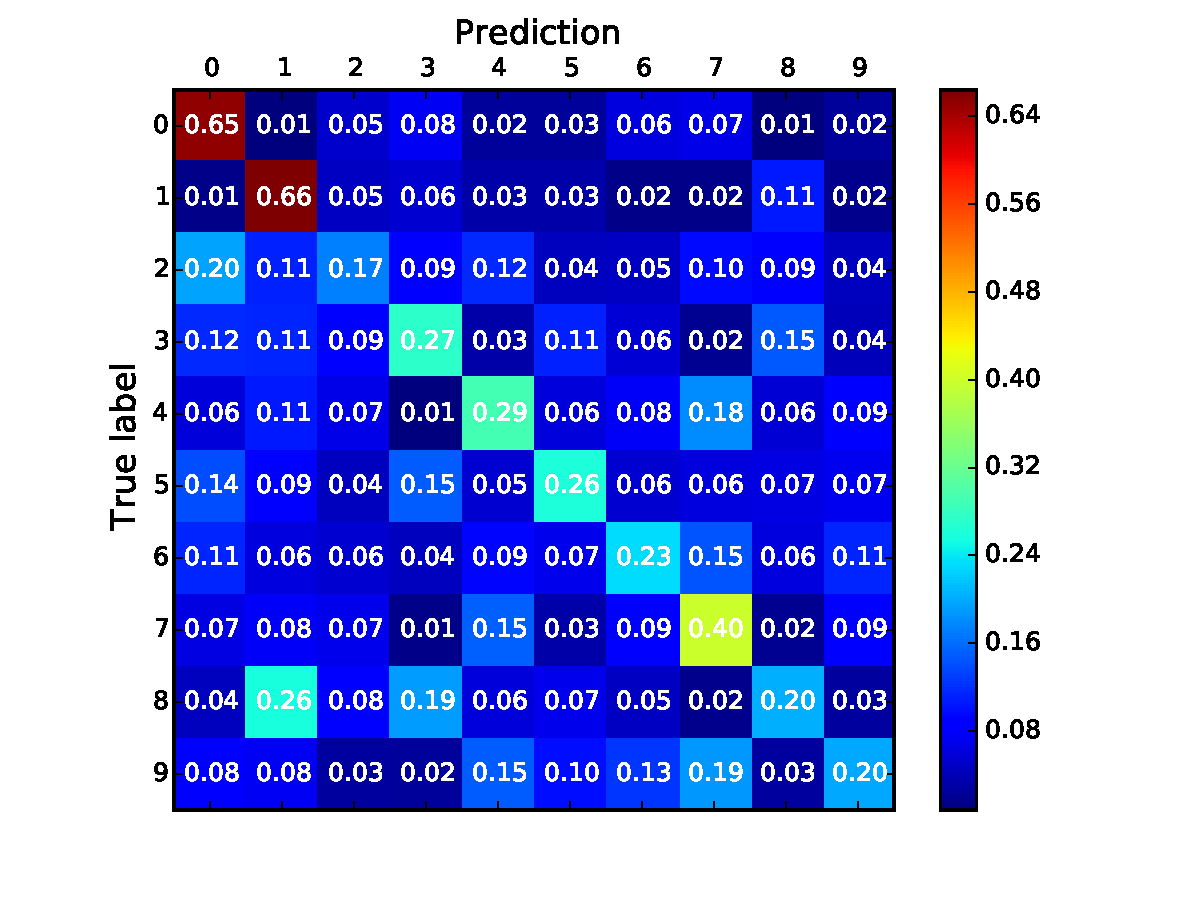
\includegraphics[width=\linewidth]{neuralnet_confusion}
  	\caption{Validation confusion matrix for fully connected neural network}
  	\label{fig:nn-conf}
\end{figure}

\subsection{Linear SVM}


\subsection{Convolutional Neural Network}
We experimented with a number of hyperparameter settings. Figure \ref{fig:convnet-compare} shows the validation accuracy of several settings. We obtained our best validation results with a convolutional neural network comprised of 4 convolution layers and one hidden layer, using a weight decay factor of 0.995, and rectified linear units (ReLU)  for all neurons--this activation function, written $$f(x) = \max(0.0, x),$$ is known to perform better than bounded activations (e.g. $\tanh$) in deep neural nets for image-related tasks, presumably because they preserve intensity information about incoming information.\cite{Nair}

\begin{figure}[h!]
	\centering
	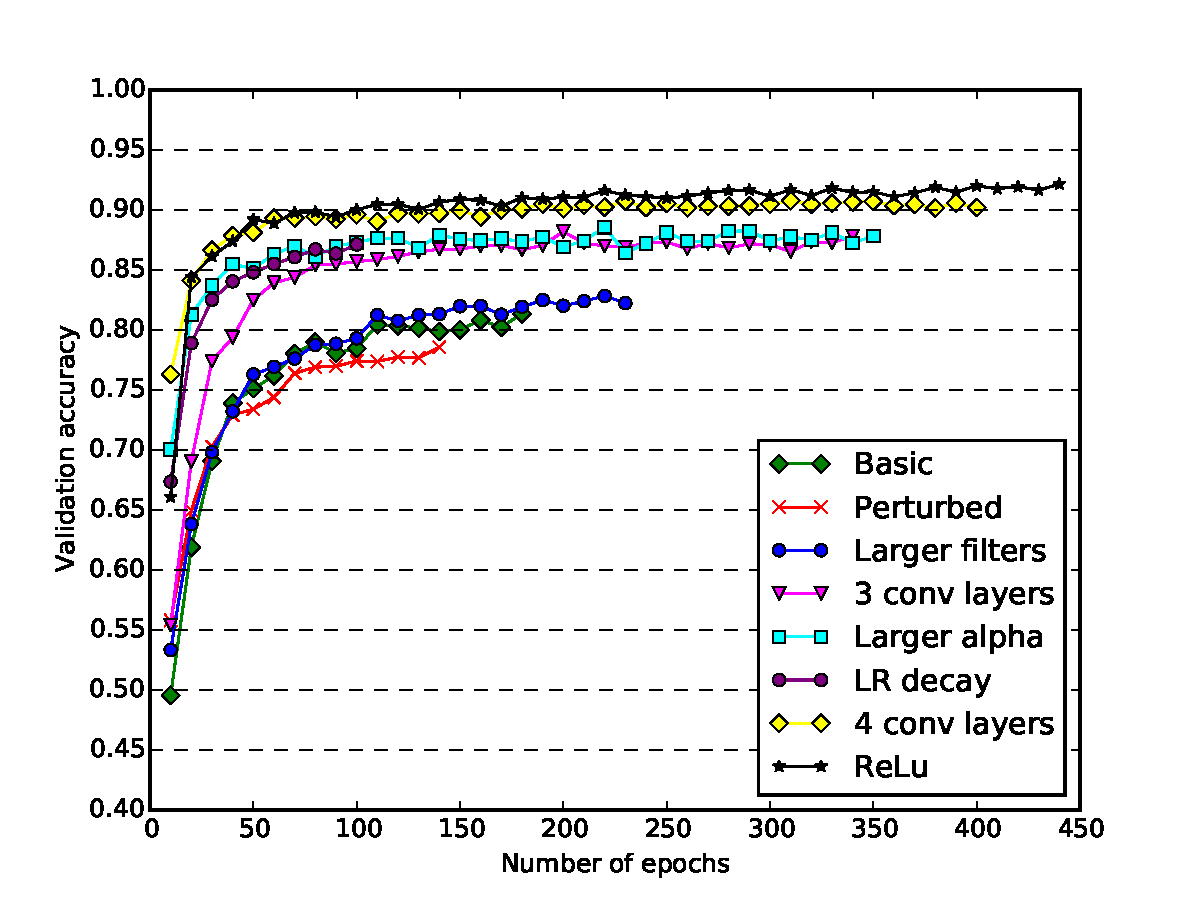
\includegraphics[width=\linewidth]{convnet_comparison}
  	\caption{Validation scores of convolutional neural network at different hyperparameter settings. Appendix \ref{sec:additional-results} elaborates on the specific hyperparameters used in the trials showed here.}
  	\label{fig:convnet-compare}
\end{figure}

Our best model, which obtained a validation accuracy of 92.64\% after 750 training epochs, achieved a test accuracy of 92.73\% on the public Kaggle leaderboard. Figure \ref{fig:convnet-architect} shows this convolutional neural network's architecture. Figure \ref{fig:convnet-confusion} displays an estimate of the model's confusion matrix using validation results at epoch 100.

 \begin{figure*}[t]
	\centering
	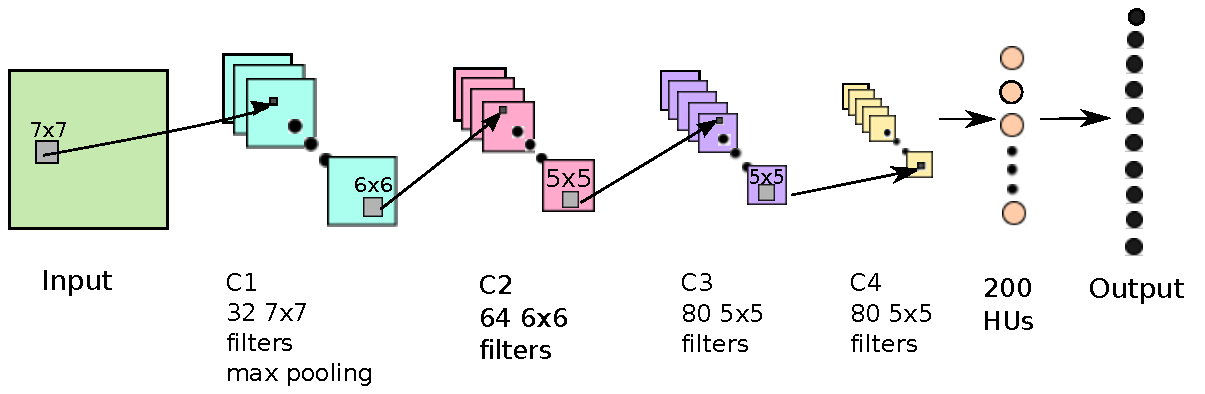
\includegraphics[width=\linewidth]{architecture.pdf}
  	\caption{Final convolutional neural network architecture. Drawn to scale.}
  	\label{fig:convnet-architect}
\end{figure*}

\begin{figure}[h!]
	\centering
	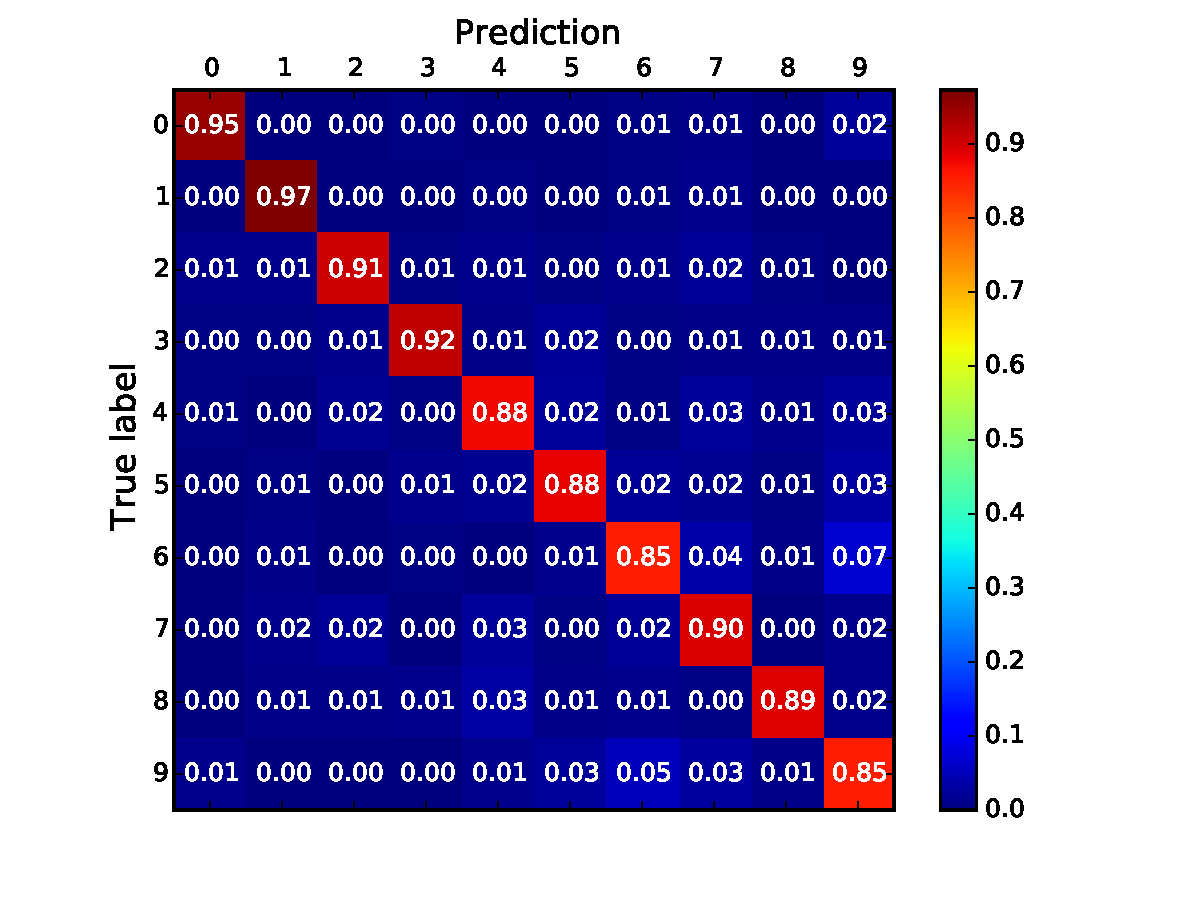
\includegraphics[width=\linewidth]{convnet_confusion.pdf}
  	\caption{Confusion matrix on validation set for convolutional neural network after 100 training epochs}
  	\label{fig:convnet-confusion}
\end{figure}


\section{Discussion}% pros/cons of approach & methodology (and alternatives)
DON'T REMOVE THE CITATIONS, I WILL USE THEM!!!!
Why is it better at classifying 0s and 1s? Interestingly, it is not due to different proportions of examples in those classes; the data is evenly distributed.

Using Gabor filters as a kernel rather than feature \cite{Sabri}

Other version of dropout \cite{Wan}

Pretraining \cite{Erhan}

Others: \cite{Rowley}, \cite{Simard}

{\bfseries We hereby state that all the work presented in this report is that of the authors.}

\bibliographystyle{abbrv}
\bibliography{references}

\newpage
\appendix
\label{appendix}

\section{Additional results}
\label{sec:additional-results}

\begin{figure}[h!]
	\centering
	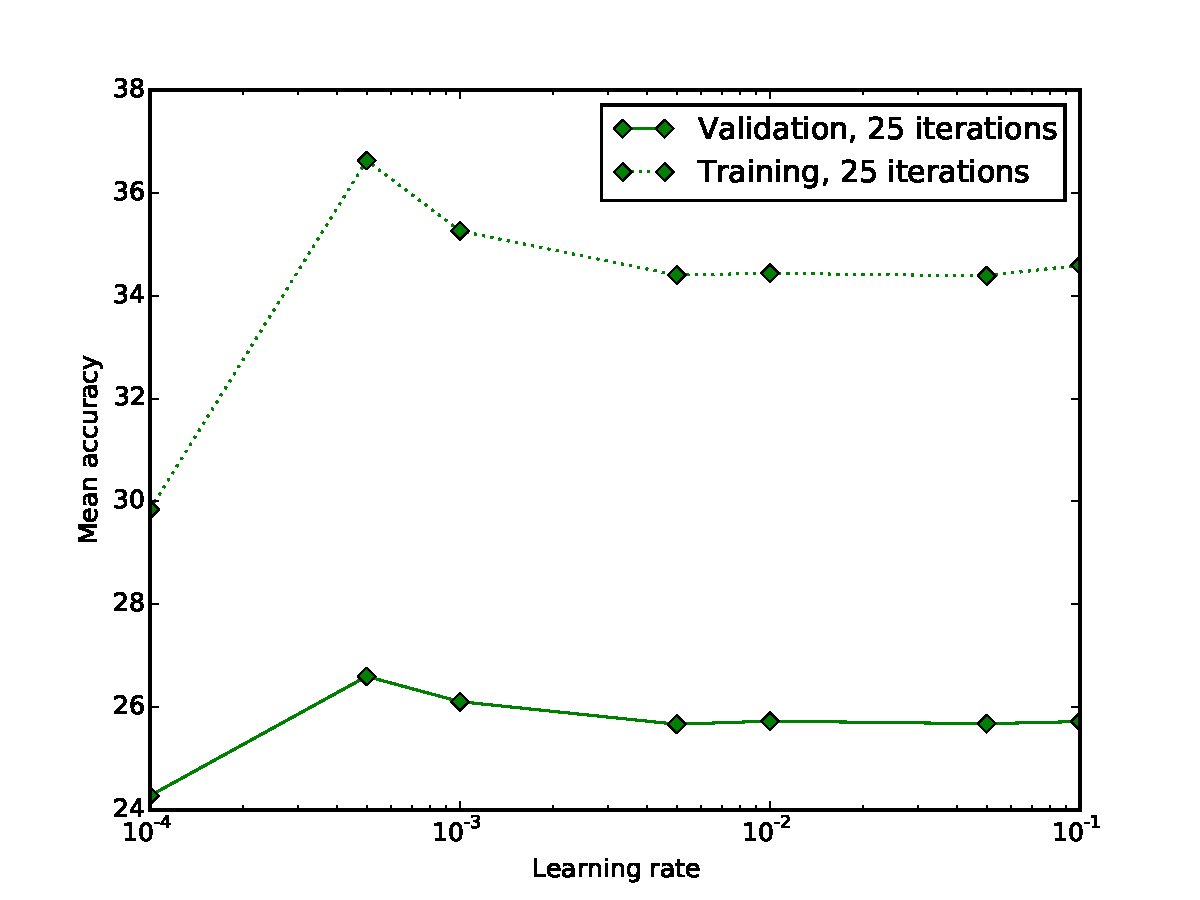
\includegraphics[width=\linewidth]{perceptron_learningrate}
  	\caption{Cross-validation over $\alpha$ with perceptron, keeping \# iterations optimal}
  	\label{fig:perc-learningrate}
\end{figure}
\begin{figure}[h!]
	\centering
	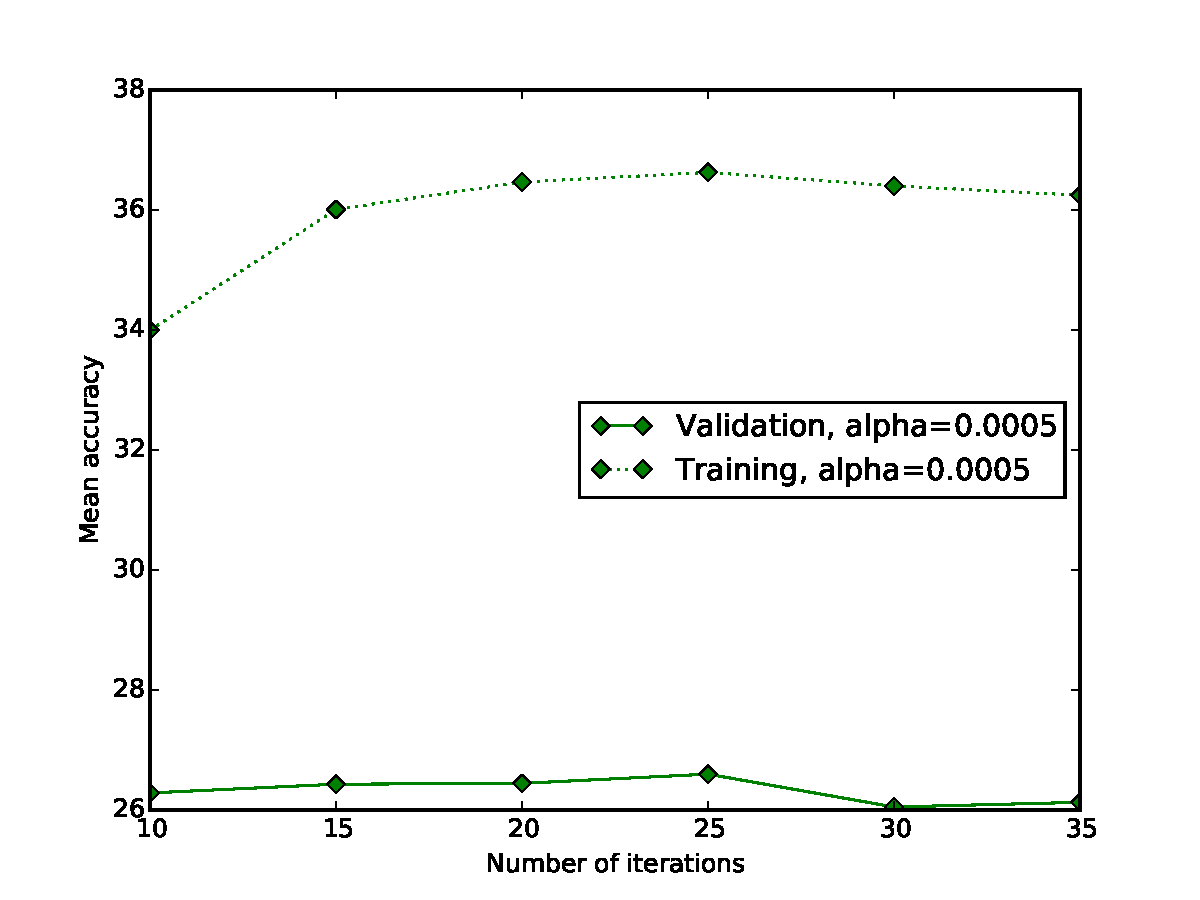
\includegraphics[width=\linewidth]{perceptron_iterations}
  	\caption{Cross-validation over \# of iterations with perceptron, keeping $\alpha$ optimal}
  	\label{fig:perc-iterations}
\end{figure}



\begin{figure}[h!]
	\centering
	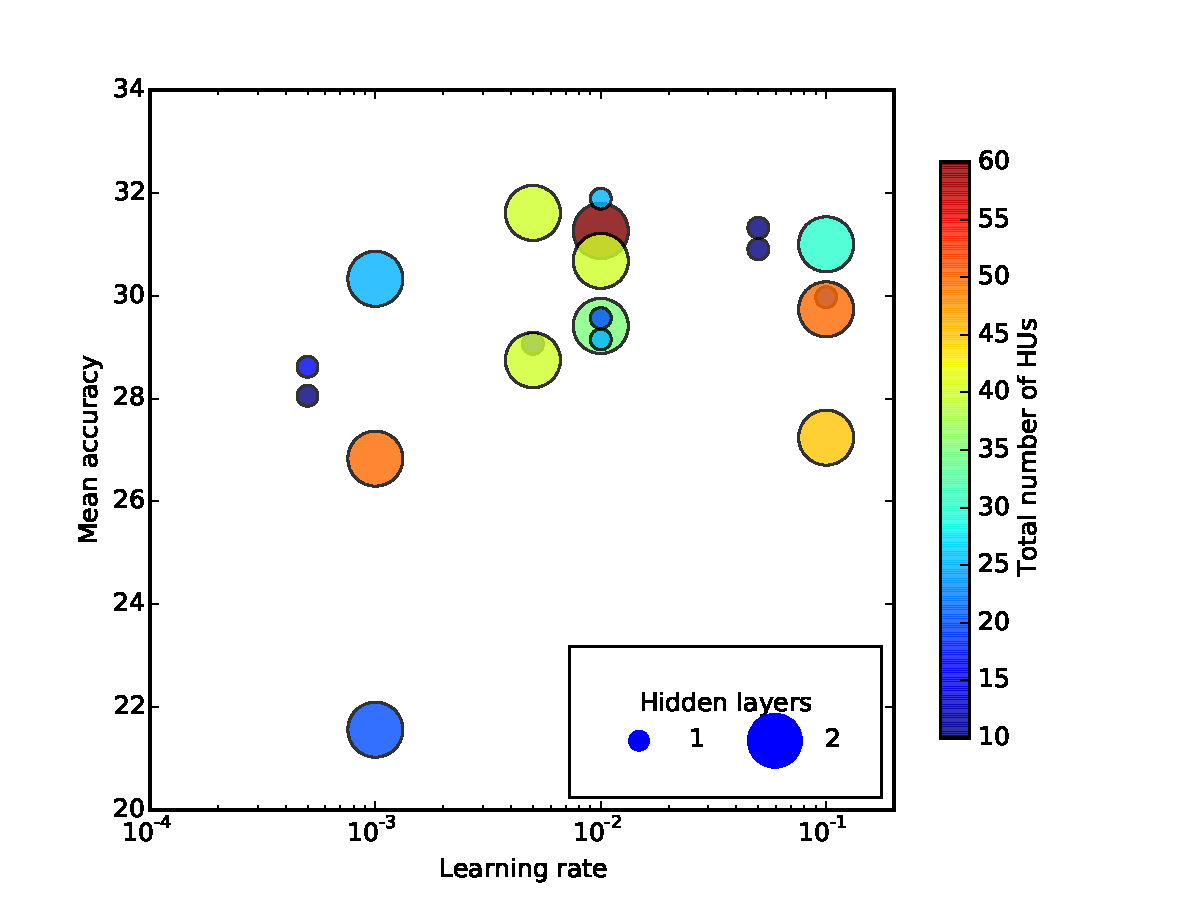
\includegraphics[width=\linewidth]{neuralnet_crossval_oddgraph}
	\caption{Cross-validation results for the neural network}
	\label{fig:nn-crossval}
\end{figure}

\begin{table*}[h!]
  \centering
  \begin{tabular}{|l|l|l|l|l|l|l|l|l|l|l|}
  \hline
    {\bfseries Label} & {\bfseries Conv} & {\bfseries Hidden} & {\bfseries Filter size} & {\bfseries \# Filters} & {\bfseries \# HUs} & {\bfseries Batch size} & {\bfseries Alpha} & {\bfseries Drop} & {\bfseries Mom} & {\bfseries Perturb}\\
    \hline \hline
    Basic & 2 & 1 & 5ds,5ds & 20,50 & 200 & 500 & 0.1 & 0.5 & No & No\\
    \hline
    Perturbed & 2 & 1 & 5ds,5ds & 20,50 & 200 & 500 & 0.1 & 0.5 & No & Yes\\
    \hline
    Larger filt & 2 & 1 & 7ds,6ds & 20,50 & 200 & 500 & 0.1 & 0.5 & No & No\\
    \hline
    3 conv & 3 & 1 & 7ds,6ds,4 & 20,50,70 & 200 & 500 & 0.1 & 0.5 & No & No\\
    \hline
    Larger $\alpha$ & 3 & 1 & 7ds,6ds,4 & 20,50,70 & 200 & 512 & 0.25 & 0.5 & No & No\\
    \hline
    LR decay & 3 & 1 & 7ds,6ds,4 & 32,64,80 & 200 & 512 & 0.2, dec 0.995 & 0.5 & No & No\\
    \hline
    4 conv & 4 & 1 & 7ds,6,5,5 & 32,64,80,80 & 200 & 512 & 0.2, dec 0.995 & 0.5 & No & No\\
    \hline
    {\bfseries ReLU} & 4 & 1 & 7ds,6,5,5 & 32,64,80,80 & 200 & 512 & 0.2, dec 0.995 & 0.5 & No & No\\
    \hline
    9 & 3 & 1 & 7ds,6ds,4 & 32,64,80 & 200 & 512 & 0.2 & 0.5 & 0.1 & No\\
    \hline
    10 & 3 & 1 & 7ds,6ds,4 & 32,64,80 & 200 & 512 & 0.2 & 0.5 & 0.9 & No\\
    \hline
    11 & 3 & 1 & 7ds,6ds,4 & 20,50,70 & 200 & 256 & 0.25 & 0.5 & No & No\\
    \hline
  \end{tabular}
  \caption{Some hyperparameters tested for convolutional neural network. Those labelled with numbers are not shown in Figure \ref{fig:convnet-compare} because they show little of interest. The notation `ds' refers to downsampling after filter application. ReLU was our best model.}
  \label{tab:convnet-params}
\end{table*}



\balancecolumns
\end{document}